\documentclass[usenames,dvipsnames]{homework}
\usepackage{cancel}
\usepackage{amsthm}
\usepackage{cleveref}
\usepackage{upgreek}
\usepackage{mathrsfs}
\usepackage{tikz}
\usepackage{units}
\usepackage{slashbox}
\usepackage{multirow}
\usepackage{listings}
%\RequirePackage[usenames,dvipsnames]{color}

\lstloadlanguages{R}

\DeclareMathOperator{\cov}{cov}

\title{Kevin Joyce}
\course{Stat 542 - Sampling - Homework 3}
\author{Kevin Joyce}
\docdate{31 October 2014}
\begin{document} 
\newcommand{\figref}[1]{\figurename~\ref{#1}}
\renewcommand{\bar}{\overline}
\renewcommand{\hat}{\widehat}
\renewcommand{\SS}{\mathcal S}
\newcommand{\HH}{\mathscr H}
\newcommand{\mom}{\widetilde}
\newcommand{\mle}{\widehat \Uptheta}
\newcommand{\eps}{\varepsilon}
\newcommand{\todist}{\stackrel{D}\longrightarrow}
\newcommand{\iid}{\stackrel{\mathrm{iid}}\sim}
\newcommand{\toprob}{\stackrel{p}\longrightarrow} \newcommand{\TTheta}{\overline{\underline \Theta} }
\newcommand{\del}{\partial}
\newcommand{\approxsim}{\overset{\cdotp}{\underset{\cdotp}{\sim}}}
\newcommand{\RSS}{\ensuremath{\mathrm{RSS}}}
\newcommand{\MSE}{\ensuremath{\mathrm{MSE}}}
\newcommand{\SE}{\ensuremath{\mathrm{SE}}}
\newcommand{\SD}{\ensuremath{\mathrm{SD}}}
\newcommand{\TSS}{\ensuremath{\mathrm{TSS}}}
\newcommand{\Var}{\ensuremath{\mathrm{Var}}}
\newcommand{\Cov}{\ensuremath{\mathrm{Cov}}}
\newcommand{\SSReg}{\ensuremath{\mathrm{SSReg}}}
\renewcommand{\a}[1]{{\color{red} \it #1}}

\begin{longproblem} In the Exxon-Valdez oil spill trial, one important issue was the amount of lost harvest of fish, shellfish, seals, etc.~suffered by native subsistence harvesters in the region. In particular, it was desired to estimate the per capita harvest loss and the total loss. Some data had been collected over the years on such harvests, both prespill and postspill.  You will analyze data from just one community for one year (1989, the spill year) and estimate total harvest and per capita harvest for this community in 1989. A random sample of 42 households out of 67 was selected from the community.  The number of individuals living in each household and the total household harvest (in pounds, estimated through detailed questioning about harvests of many individual species) were recorded.

The data are available on the website in the file \texttt{harvest.csv}.  The resulting data frame has two variables: \texttt{size} (the number of people in household) and \texttt{harvest} (in pounds).
\end{longproblem}

\subproblem{ Estimate the per capita harvest for this community.  Attach a standard error to your estimate and calculate a \unit[95]{\%} confidence interval. }
\begin{solution}
 % $$
 %   \hat\mu = \frac NM \bar y \approx 305.84\text{ pounds per person with } \SE(\hat\mu) = \frac 1M \sqrt{N(N-n) \frac{s_u^2}n} \approx 29.91\text{ pounds.}
 % $$
 % A normal based confidence interval for $\hat\mu$ is given by $\big(247.22,\,364.45\big)$ pounds.
 % This is a cluster sample plan with households as the cluster.  Denote $y_i$ as the household harvest in pounds, and using totoal population $M=190$ of the region, we can estimate the per capita harvest by
 Denote the harvest per household $y_i$ and the size of each household $M_i$.  Since we do not (at this point) know the total population, if we assume that the amount harvested per household is roughly linear with the amount of people in the household, we can use a ratio estimator to estimate the population per capita harvest
$$
  \hat\mu_r = \frac{\ds{\sum_{i=1}^n y_i}}{\ds{\sum_{i=1}^n M_i}} \approx 282.4 \text{ pounds. }
$$ 
  If we denote the average household size $\bar M$, the linearized estimate for the variance of $\hat\mu_r$ is given by
  $$
    \Var(\hat\tau) =  \left(\frac {N-n}{\bar M^2N}\right) \frac{s_u^2}{n},
  $$
  from which we can estimate the standard error of $\hat\mu_r$ by estimating $\bar M^2$ with $(\frac 1n\sum M_i)^2$. We obtain
  $$
    \SE(\hat\tau)\approx 24.36
  $$
  A normal based confidence interval for $\hat\mu_r$ is given by $\big(234.6,\,330.1\big)$ pounds.
  
\end{solution}

\subproblem{ Estimate the total harvest for the community.  Attach a standard error to your estimate and calculate a \unit[95]{\%} confidence interval.}
\begin{solution}
  We estimate the total harvest with
  $$
    \hat\tau = N\bar y \approx 58\,109 \text{ pounds with } \SE(\hat\tau) =  \sqrt{N(N-n) \frac{s_u^2}n} \approx 5\,682 \text{ pounds. }
  $$
  A normal based confidence interval for $\hat\tau$ is given by $\big(46\,972,\,69\,246\big)$ pounds.
\end{solution}

\subproblem{ Now suppose the total number of individuals in the community is known to be 190 (do not use this information in part b).  Estimate total harvest using both ratio and regression estimation and calculate SE's.  Compare these results with your result in (b); is there much of an improvement?  Which seems more appropriate based on a plot of the data: ratio or regression estimation? }
\begin{solution}
  For the ratio estimator, we merely scale the answers from part (a) by the total population.
  \begin{align*}
    \hat\tau_r = M r = M\frac{\sum y_i}{\sum M_i} &\approx 53\,652 \text{ pounds }\\ 
    \text{ with } \SE(\hat\tau_r) \approx M\sqrt{\left(\frac {N-n}{\bar m^2N}\right) \frac{s_u^2}{n}} &\approx 4\,628\text{ pounds }
  \end{align*}
  where $s_r^2 = \frac 1{n-1}\sum(y_i - rM_i)^2$. Although, since we now know the true population, $M$, we can estimate more precicely the standard error with
  $$
    \text{ with } \SE(\hat\tau_r) \approx \sqrt{N\left(\frac {N-n}{N}\right) \frac{s_u^2}{n}} \approx 5012 \text{ pounds. }
  $$
  Note that this is \emph{larger} than the estimate that does not take $M$ into account.  This may be due to the bias of that estimator.

  The regression estimator is given by
  \begin{align*}
    \hat\tau_{reg} = N\hat\mu_{reg} = Na + Mb  &\approx 54\,230\text{ pounds } \\
    \text{ with } \SE(\hat\tau_{reg}) \approx M\sqrt{ \frac{N-n}N \frac{s_{reg}^2}{n}} &\approx 5\,058\text{ pounds }
  \end{align*}
  where $a$ and $b$ are estimates of the linear least-squares fit for the population household size versus the population household harvest and $s_{reg}^2 = \frac1{n-2}\sum(y_i-a-bx_i)^2$.

\begin{minipage}{.48\textwidth}
  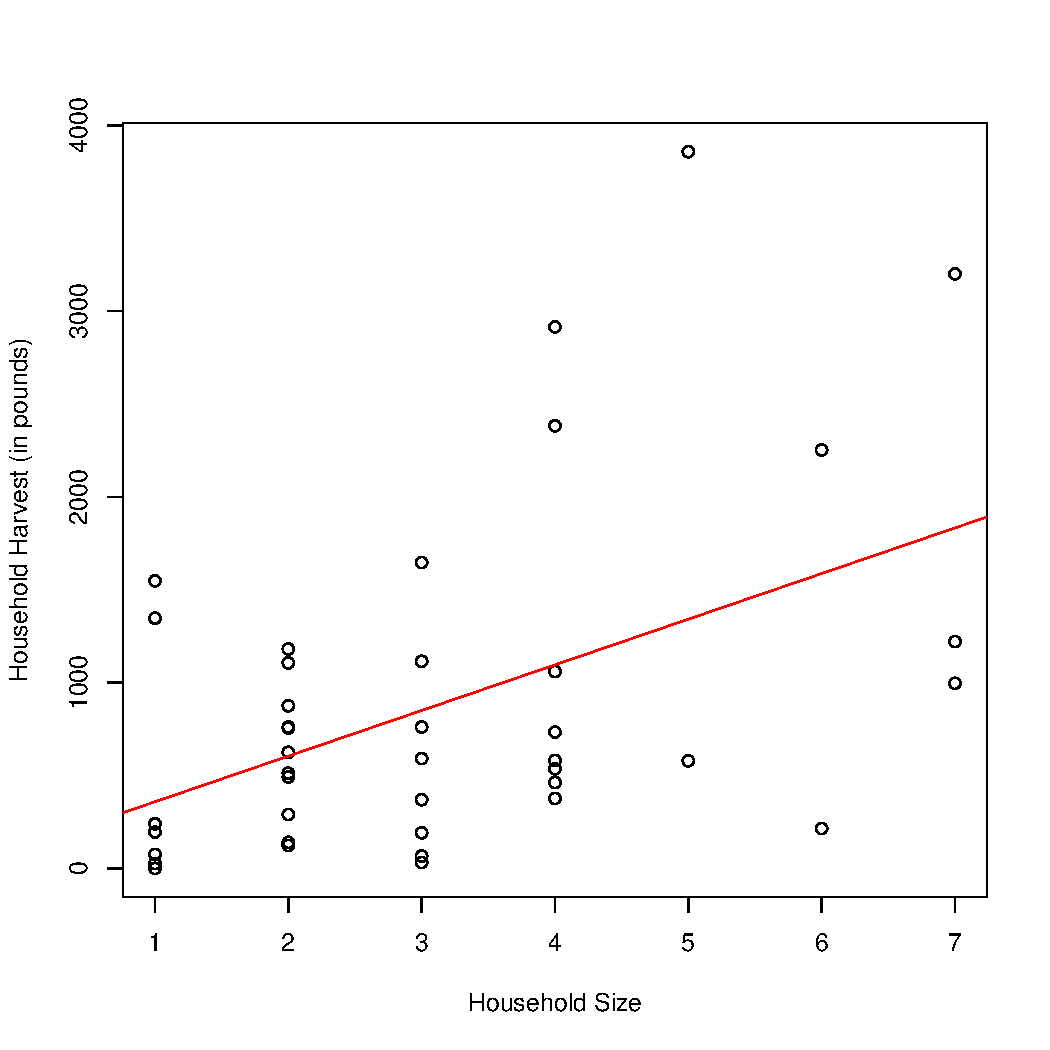
\includegraphics[width=\textwidth]{harvest_ratio.pdf}
\end{minipage}
\begin{minipage}{.48\textwidth}
  It appears that there is a moderate relationship between household size and harvest, and there is an appreciable reduction in the standard errors from part b.  It appears that estimating the extra parameter in the regression estimate doesn't offer a reduction in the standard error (although this may be due to the quality of the estimator for $\Var(\hat \tau_{reg})$). From the plot to the left, there doesn't seem to be much of an indication for estimating an intercept.
\end{minipage}
\end{solution}

\begin{longproblem}
  Kruuk et al.~(1989) used a stratified sample to estimate the number of otter dens (called holts) along the coastline of Shetland, UK.  The coastline (except for parts that were predominantly buildings) was divided into 237 \unit[5]{km} sections and each section was assigned to one of four terrain types.  A random sample of sections within each stratum were chosen for counting. In each section chosen, researchers counted the number of otter dens in a \unit[110]{m} wide strip along the coast.  The data are in the file \texttt{otters.csv}.  The population and sample sizes for the strata are given in the table below.  Estimate the total number of otters along the coast of Shetland, along with a standard error and a \unit[95]{\%} confidence interval.  Note: use the \texttt{tapply} command in \texttt{R} to compute the variance (or any other function) of the observations by stratum. 
  \begin{center}
  \renewcommand{\arraystretch}{1.3}
  \begin{tabular}{l c c}
  Stratum			      & Total Sections  & Sections Counted \\ \hline
  \textbf{1} Cliffs over \unit[10]{m} & 89              & 19               \\
  \textbf{2} Agriculture              & 61              & 20               \\
  \textbf{3} Not 1 or 2, peat         & 40              & 22               \\
  \textbf{4} Not 1 or 2, nonpeat      & 47              & 21               \\ \hline
  \end{tabular}
  \end{center}
\end{longproblem}
\begin{solution}
  Denote each stratum with $h=1,2,3,4$, then an estimate of the total number of holts is
  $$
    \hat\tau = \sum_{h=1}^4 N_h\bar y_h \approx 985\text{ holts with }\SE(\hat\tau) = \sqrt{\sum_{h=1}^4 N_h^2\left(1-\frac{n_h}{N_h}\right) \frac{s_h^2}{n_h}} \approx 74\text{ holts.}
  $$
  Using a normal approximation, a \unit[95]{\%} confidence interval is given by $\big(840,\,1130\big)$. On the other hand (thanks to Grant Swicegood for pointing this out to me), if we take estimation of each $s_i$ into account and use the Satterthwaite d.f. approximation to use a $t$ distribution, then the confidence interval is $\big(837,\, 1132\big)$. 
\end{solution}

\begin{longproblem}
  Using aerial photographs, a forester stratifies a \unit[400]{acre} forest into three strata, and plans to sample each stratum using \unit[0.1]{acre} plots to estimate the total cubic foot volume of timber.  From past surveys, he has information on the range of volumes (largest minus smallest volumes likely to occur per plot) and cost in dollars for surveying a plot in each stratum.  These data can be used in planning the survey and are summarized below.

  \begin{center}
  \renewcommand{\arraystretch}{1.3}
  \begin{tabular}{l c c c}
  \hline
  Stratum			         & Acreage & Range & Cost $(c_i)$ \\ \hline
  1. Small Pines (trees 50-70 feet tall) & 180     & 80    & 20           \\
  2. Large Pines (trees 70-90 feet tall) & 70      & 120   & 25           \\
  3. Mixed Pine -- hardwood swamp        & 150     & 200   & 35           \\ \hline
  \end{tabular}
  \end{center}
  Suppose he wants to estimate the total cubic foot volume on the tract with an allowable error of 20,000 cubic feet at the \unit[95]{\%} confidence level. (On a per plot basis, the allowable error would be 5 cubic feet.)  Compute equal, proportional, optimal equal cost (Neyman), and optimal unequal cost allocations and compute the total cost of each allocation.  Briefly discuss.

\newpage
\end{longproblem}

\begin{solution}
Based on the Finite Central Limit Theorem, let us assume that the stratified mean estimator $\bar y_{st}$ is normally distributed, centered at the mean cubic foot volume per plot $\mu$, , with variance (derived in the notes)
$$
  \Var(\bar y_st) = \sum_{h=1}^3\left(\frac{N_h}{N} \right) \left( \frac{N_h - n w_h}{N_h}\right) \frac{\sigma^2_h}{w_h}  
$$
where $N=4000$ possibly sampled plots, and $w_h$ is the proportion of $N_h$ (the acreage $\times$ 10)  to be sampled.  We assume that within each stratum the standard deviation is given by $3 \sigma_h = \frac{R_h}2$, where $R_h$ is the range of volumes given (based on the fact that $P(|X|<2\sigma) \approx .997$ for $X$ normally distributed with standard deviation $\sigma$).
Solving the margin of error equation for $n$ where $z$ is the $.975$ quantile of the standard normal distribution, we have
$$
  n = \frac{\ds{\sum_{h=1}^3\left(\frac{N_h}{N}\right)^2\frac{\sigma_h^2}{w_h}}}{\ds{\frac{d^2}{z^2} + \frac 1N \sum_{h=1}^3 \left( \frac{N_h}{N} \right)\sigma_h^2}}.
$$
For each statification scheme, aside from optimal unequal cost, we can substitute $w_h$ associated with a given allocation scheme into this formula.  In the case of unequal cost, the weights are given implicitly in terms of the total added cost $c^*=c-c_0=\sum n_h c_h$.  It turns out that $c^*$ has a similar formula for the optimal $n$ in the other cases, so after solving for $c^*$ we obtain $n=\sum n_h = \sum c^*w_h$.  

In the following table we summarize the total sample size calculation for various statified weighting schemes (see notes).
\begin{center}
\renewcommand{\arraystretch}{2.5}
\begin{tabular}{l l|c c c|c c}
Scheme		      & $w_h$					 &$n_1$ & $n_1$& $n_1$& $n$  & $c$    \\ \hline
Equal Weights         & $w_h=\ds{\frac 1L}$                       & 31 & 31 & 31 & 93 & \$2480 \\
Proportional Weights  & $w_h=\ds{\frac{N_h}N}$                    & 38 & 15 & 32 & 85 & \$2255 \\
								 
Optimal Equal Cost    & $w_h=\ds{\frac{N_h\sigma_h}                                               
			        {\sum N_k\sigma_k}}$              & 20 & 12 & 41 & 73 & \$2135 \\
Optimal Unequal Cost  & $^*w_h=\ds{\frac{c^*}{n}                 
				\frac{N_h\sigma_h/\sqrt{c_h}}    
			        {\sum N_k\sigma_k/\sqrt{c_k}}}$	  & 24 & 12 & 38 & 74 & \$2110 \\ \hline
\end{tabular}
\end{center}

Note that as more information is included in the analysis, the total cost of the study goes down.  For the optimal variance allocation, note that the mixed pine is sampled more heavily due to a wider range, but when cost constraints are taken into account less of them are sampled in favor of the cheaper strata.
\end{solution}

\begin{longproblem}
A nursery manager wants to estimate the average height of seedlings in a large field that is divided into 25 plots that vary slightly in size.  She believes the heights are fairly constant throughout each plot, but may vary considerable from plot to plot.  Although this seems to indicate the need for a stratified random sample, for time and logistical reasons, she decides to use a two-stage sample, where with the low variability within a plot, she decides to sample \unit[10]{\%} of the trees within each of 5 plots.  The data are given in the table below.  Estimate the average height of seedlings in the field, give the standard error, and find an approximate \unit[95]{\%} confidence interval for the mean.  [Problem taken from page 304, Scheaffer, Mendenhall, \& Ott.]

  \begin{center}
  \renewcommand{\arraystretch}{1.3}
  \begin{tabular}{c c c c c c c c c}
  \hline
       & Number of & Number of		& \multicolumn{6}{c}{Heights of Seedlings} \\ 
  Plot & Seedlings & Seedlings Sampled  & \multicolumn{6}{c}{(in inches)}          \\ \hline
  1    & 52        & 5                  & 12 & 11 & 11 & 10 & 13 &    \\
  2    & 56        & 6                  & 10 &  9 &  7 &  8 &  8 & 10 \\
  3    & 60        & 6                  &  6 &  5 &  7 &  5 &  6 &  4 \\
  4    & 46        & 5                  &  7 &  8 &  6 &  7 &  6 &    \\
  5    & 49        & 5                  & 10 & 11 & 13 & 12 & 12 &    \\\hline
  \end{tabular}
  \end{center}
\end{longproblem}
\begin{solution}
  In this two-stage sample, we do not know the total number of seedlings, hence
  we cannot use the unbiased estimator for the average height per seedling.  
  If we denote $y_i$ as the total height of seedlings in the $i$th group of $n=5$, 
  we can estimate the average height per seedling with the ratio of an estimate of the average height per plot with an estimate of 
  the average number of seedlings per plot. I.e. 
  $$
    \hat\mu_r = \frac{\hat\mu_1}{\bar m} = \frac{\hat y_i/n}{\ds{\frac 1n\sum_{i=1}^n M_i }} = \frac{\ds{\sum_{i=1}^n M_i\bar y_i }}{\ds{\sum_{i=1}^n M_i }} \approx 8.705\text{ inches. }
  $$
  Denote $N$ as the total number of plots, then the linearized variance is
  $$
    \Var(\hat\mu_r) \approx \left(1-\frac nN\right) \frac 1{\bar M^2n} \left(\frac 1{N-1} \sum_{i=1}^N(y_i - M_i\hat\mu)^2\right) + \frac{1}{N\bar M^2n} \sum_{i=1}^n M_i (M_i - m_i) \frac{\sigma_i^2}{m_i},
  $$
  from which we can estimate a standard error by estimating $y_i$ with $\hat y_i$, $\bar M$ with $\bar m = \frac 1n\sum M_i$, $\mu$ with $\hat\mu_r$ and $\sigma_i^2$ with $s_i^2 = \frac{1}{n-1}\sum (y_{ij} - \bar y_i)^2$. The result is
  \begin{align*}
    \SE(\hat\mu_r) 
    &\approx \sqrt{\left(1-\frac nN\right) \frac 1{\bar M^2n} \left(\frac 1{n-1} \sum_{i=1}^n(y_i - M_i\hat\mu)^2\right) + \frac{1}{N\bar M^2n} \sum_{i=1}^n M_i (M_i - m_i) \frac{\sigma_i^2}{m_i}} \\
     &\approx \sqrt{1.108362 + 0.00792}\\
     &\approx 1.11\text{ inches. (Continued on next page)}
  \end{align*}
  \newpage
  Note that the computation is dominated by the first ``between-group'' variance term.  This is not surprising due to the small number of primary units sampled $n=5$.  
  Due to the small sample size, we use a conservative \unit[95]{\%} confidence interval based on a $t$ distribution with $4$ degrees of freedom: $\big(5.63,\, 11.78 \big)$. 
  \vspace{-2em}
\end{solution}


\begin{longproblem}An auditor wishes to sample sick-leave records of a large firm in order to estimate the average number of days of sick leave per employee over the past quarter.  The firm has eight divisions, with varying numbers of employees per division.  Since the number of days of sick leave used within each division should be highly correlated with the number of employees, the auditor decides to sample $n=3$ divisions with probabilities proportional to the number of employees.  The data are given in the table below.

\begin{center}
\renewcommand{\arraystretch}{1.3}
\begin{tabular}{c | c c c c c c c c } 
Division	& 1    & 2   & 3    & 4   & 5    & 6    & 7   & 8    \\\hline
\# of Employees & 1200 & 550 & 2240 & 860 & 2800 & 1910 & 390 & 3200 \\
\end{tabular}
\end{center}
\end{longproblem}

\subproblem{ Explain how, using a random number table or generator, such a sample could be taken.  You do not need to do it -- just explain it. }
\begin{solution}
  Let $p_i$ be the proportion of employees in the $i$th division.  If we let $D$ be the number of the division choosen so that the probability of selection is equal to $p_i$, then the cummulative probability function for $D$ is $c_n:=P(D\le n) = \sum_{i=1}^n p_i$. Assuming we have $u_1,u_2$ and $u_3$ realizations from a uniform distribution over $[0,1]$, select $i$ such that $c_{n-1} < u_i \le c_{n}$ for $i=1,2,3$.  Using a theorem from probability, $n(i)$ are realizations from the distribution of $D$. Pictorally,
  \begin{center}
  \begin{tikzpicture}
  \draw (0,0) -- (10,0);   
  \draw (0pt,2pt) -- (0pt,-2pt) node[below] {\footnotesize $0$};
  \foreach[count=\i] \x in {0.913, 1.331, 3.034, 3.688, 5.817, 7.270, 7.567, 10.000} {
    \draw[shift={(\x,0)}] (0pt,2pt) -- (0pt,-2pt) node[below] {\footnotesize $c_{\i}$};
  }
  \draw (.7,0) circle (1pt) node[above] {\footnotesize $u_1$}; 
  \draw (2,0) circle (1pt) node[above] {\footnotesize $u_2$}; 
  \draw (9,0) circle (1pt) node[above] {\footnotesize $u_3$}; 
  \end{tikzpicture} 
  \end{center}

\end{solution}

\subproblem{ Suppose now that such a sample is taken where divisions 1, 3, and 8 are selected, and that the total number of sick days used by the three sampled divisions during the past quarter are, respectively,
$$
  y_1 = 2410,\quad y_2=4320,\quad y_3=5790.
$$
Estimate the average number of sick days used per person for the entire firm, and give the corresponding standard error.
}

\begin{solution} 
  Denote the division size $M_i$, and $y_i$ the number of sick days, we can estimate using the Hansen-Hurwitz estimator:
  $$
    \hat\mu_p = \frac 1M \hat\tau_p = \frac 1{Mn} \sum_{i=1}^n \frac{y_i}{p_i} = \frac{1}{n}\sum_{i=1}^n \frac{y_i}{M_i} = \frac 13\left\{\frac{2410}{1200} +  \frac{4320}{2240} + \frac{5790}{3200}\right\} \approx 1.92 \text{ hours. }
  $$
  We estimate the standard error with ($\bar y_i = y_i/M_i$)
  $$
    \SE(\hat\mu_p) = \sqrt{ \frac1{n(n-1)}\sum_{i=1}^n(\bar y_i - \hat\mu_p)^2} \approx 0.0578\text{ hours. }
  $$
  %The normal based confidence interval is $\big(1.67,\,2.16\big)$. Although, the sample size here is fairly small ($n=3$), and a normal approximation for $\hat \mu_p$ might not be appropriate, although what alternative distribution to use for this estimator is not obvious. Previous comments about the trustworthiness of this small samply estimator apply.

\end{solution}

\problem{Show that in two-stage sampling with equal-sized primary units, that if $m$ secondary units will be sampled within each primary unit, then the number of primary units $n$ required to estimate the population mean per secondary unit to within $d$ with probability \unit[$100(1-\alpha)$]{\%} is given as
$$
  n = \frac{\ds{\sigma_b^2 + \left(\frac{\bar M-m}{\bar M}\right) \frac{\sigma_w^2}{m}}}{\ds{\frac {d^2}{z^2} + \frac{\sigma_b^2}{N}}}.
$$
}
\begin{solution}
  It was shown in the notes that the variance of this estimator for the population mean per secondary unit was given as
  $$
    \Var(\hat \mu) = \left(1 - \frac nN\right) \frac{\sigma_b^2}{n} + \left(\frac {\bar M - m}{\bar M}\right) \frac{\sigma^2w}{m\cdot n}.
  $$
  Based on the Finite Population Central Limit Theorem, if we assume that $\hat\mu$ is normally distributed, then the margin of error, say $d$, for a $100(1-\alpha)\%$ is given by
  $$
    d = z \sqrt{\Var(\hat\mu)}
  $$
  where $z$ is the $1-\frac \alpha 2$ quantile for the standard normal distribution. Then,
  \begin{align*}
    \frac{d^2}{z^2} 
    &= \frac{\sigma_b^2}{n} - \frac{\sigma_b^2}{N} + \frac 1n\left( \frac {\bar M - m}{\bar M}\right) \frac{\sigma^2w}{m}\\
    &= \frac 1n\left(\sigma_b^2 + \left(\frac {\bar M - m}{\bar M}\right) \frac{\sigma^2w}{m}\right)  - \frac{\sigma_b^2}{N}  \\
    \intertext{ so }
    n&= \left( \frac{d^2}{z^2} +  \frac{\sigma_b^2}{N}\right)^{-1}\left(\sigma_b^2 + \left(\frac {\bar M - m}{\bar M}\right) \frac{\sigma^2w}{m}\right)
  \end{align*}

\end{solution}

\newpage 

\problem{ Use conditional expectations to solve the following problems. }

\subproblem{ Derive the variance of a geometric random variable (we derived the expected value by conditioning in class). }
  Let $X$ be a geometrically distributed random variable with probability $p$.  That is, for $T_i \iid \text{Bernoulli}(p)$, $X$ is the first $i$ such that $T_i = 1$. If we condition on $T_1$, then
  $$
    \Var(X|T_1 = 0) = \Var(X+1) = \Var(X)
  $$
  since $X$ ``has no memory'' of the first trial. On the other hand, 
  $$
    \Var(X|T_1 = 1) = 0
  $$
  since $(X|T_1=1) = 1$ is completely determined.  Now, thinking of $g(t) = \Var(X|T_1=t)$, we can calculate 
  $$
    E\Big[ \Var(X|T_1) \Big] = E(g(T_1)) = (1-p)\Var (X) + \cancel{p\cdot0}.
  $$
  Thinking along similar lines, $E(X|T_1)$ is a random variable whose mean is $E(X) = 1/p$ that takes on $1/p + 1$ with probabilty $1-p$ and $1$ with probability $p$ (this was done in class). Hence
  $$
    \Var\Big[ E(X|T_1) \Big] = (1-p)(1/p + 1 - 1/p)^2 + p(1 - 1/p)^2 = (1-p) + p\frac{(1-p)^2}{p^2} = \frac{1-p}p. 
  $$
  The ``EVVE'' law for conditional variance gives
  $$
    \Var(X) = E\Big[ \Var(X|T_1) \Big] + \Var\Big[ E(X|T_1) \Big] = (1-p)\Var(X) + \frac{1-p}p \iff \Var(X) = \frac{1-p}{p^2}.
  $$

\subproblem{ What is the expected number of rolls of a fair die until you have obtained two \emph{consecutive} 6's? }
Let $X$ be the number of rolls until two consecutive sixes are rolled.  If we denote event of obtaining a six on the $i$th roll $T_i$, then it can be thought of as a Bernoulli trial with probability $\frac 16$.  Conditioning on $T_1$, we have 
$$
  E(X|T_1 = 0) = E(X+1) = E(X) + 1
$$
To evaluate $E(X|T_1=1)$, we further condition on $T_2$ so that
$$
  E(X|T_1 = 1,\,T_2=0) = E(X+2) = E(X) + 2
$$
and
$$
  E(X|T_1=1,\,T_2=1) = 2
$$
since that event is completely determined to be 2. Now, thinking of $g(t) = E(X|T_1 = 1,\,T_2=t)$, we can calcuate the expectation
$$
  E(X|T_1 = 1) = E\Big[ E(X|T_1=1,\,T_2) \Big] = \frac 16\cdot 2 + \frac 56 (E(X) + 2) = 2 + \frac 56 E(X).
$$
Using similar reasoning,
$$
  E(X) = E\Big[ E(X|T_1) \Big] = \frac 56(E(X) + 1) + \frac16\left(\frac 56 E(X) + 2\right) \iff E(X) = 42.
$$

\lstset{language=R,
	frame=shadowbox,
	basicstyle=\small\ttfamily, % the size of the fonts that are used for the code
  	backgroundcolor=\color{white},  % choose the background color. You must add \usepackage{color}
  	showspaces=false,               % show spaces adding particular underscores
  	showstringspaces=false,         % underline spaces within strings
  	showtabs=false,                 % show tabs within strings adding particular underscores
  	rulecolor=\color{black},        % if not set, the frame-color may be changed on line-breaks within not-black text (e.g. commens (green here))
  	tabsize=2,                      % sets default tabsize to 2 spaces
  	captionpos=b,                   % sets the caption-position to bottom
  	breaklines=true,                % sets automatic line breaking
  	breakatwhitespace=false,        % sets if automatic breaks should only happen at whitespace
  	keywordstyle=\color{RoyalBlue},      % keyword style
  	commentstyle=\color{YellowGreen},   % comment style
  	stringstyle=\color{ForestGreen}      % string literal style
	}
\begin{lstlisting}
> source('problem1.r',echo=T) 
> ##################################
> # Problem 1
> ##################################
> d = read.csv('harvest.csv')
> N = 67
> M = 190
> n = nrow(d)

> #(muhat = N/M*mean(d$harvest))
> #(se_muhat = 1/M*sqrt(N*(N-n)*var(d$harvest)/n))
>
> # part (a)
> (murhat = sum(d$harvest)/sum(d$size))
[1] 282.377

> sr2 = sum((d$harvest - murhat*d$size)^2)/(n-1)
> (se_murhat = sqrt( (1-n/N)/mean(d$size)^2 * sr2/n ))
[1] 24.35694

> (murhat_ci = murhat + c(-1,1)*qnorm(.975)*se_murhat)
[1] 234.6382 330.1157

> # part (b)
> (tauhat = N*mean(d$harvest))
[1] 58109.14

> (se_tauhat = sqrt(N*(N-n)*var(d$harvest)/n))
[1] 5682.249

> (tauhat_ci = tauhat + c(-1,1)*qnorm(.975)*se_tauhat)
[1] 46972.14 69246.15

> # part (c)
> plot(d$size,d$harvest,xlab="Household Size",ylab="Household Harvest (in pounds)") 
> out = lm(d$harvest ~ d$size) 
> abline(out,col="red")

> (taurhat = M*murhat)
[1] 53651.62

> (se_taurhat = M*se_murhat)
[1] 4627.819

> (se2_taurhat = sqrt(N^2*(1-n/N) * sr2/n ))
[1] 5012.311

> (taureghat = N*out$coefficients[1] + M*out$coefficients[2])
(Intercept)
   54230.49

> sreg2 = sum(out$residuals^2)/(n-2)
> (se_taureghat = N*sqrt((1-n/N) * sreg2/n))
[1] 5058.067

> source('problem2.r',echo=T) 
> ######################################
> # Problem 2
> ######################################
> otters = read.csv('otters.csv') 
> nh = table(otters$Habitat) 
> Nh = c('1'=89,'2'=61,'3'=40,'4'=47) 
> ybarh = tapply(otters$Holts,otters$Habitat,mean)  
> sh2 = tapply(otters$Holts,otters$Habitat,var) 
> (tauhat = sum(Nh*ybarh))
[1] 984.7142

> (se_tauhat = sqrt(sum(Nh^2*(1-nh/Nh)*sh2/nh)))
[1] 73.92099

> (tauhat_ci = tauhat + c(-1,1)*se_tauhat*qnorm(.975))
[1]  839.8317 1129.5967

> ah = Nh*(Nh-nh)/nh
> satterthwaite_df = sum(ah*sh2)^2/sum((ah*sh2)^2/nh-1)
> (tauhat_sat_ci = tauhat + c(-1,1)*se_tauhat*qt(.975,satterthwaite_df))
[1]  837.3809 1132.0476

> source('problem3.r',echo=T) 
> #####################################                                                                                                                                                  
> # Problem 3                                                                                                                                                                            
> #####################################                                                                                                                                                  
> N = 4000                                                                                                                                                                               
> Nh = c(1800,700,1500) 
> Rh = c(80,120,200) 
> ch = c(20,25,35) 
> sigh = (Rh/6) # Using P(|X|< 3 sig) = .997 
> d = 5 
> total_n = function(wh) { # Use the general equation and just input wh
+   sum( (Nh*sigh)^2/wh ) / ( (N*d/qnorm(.975))^2 + sum(Nh*sigh^2) )
+ }

> equal_wh = rep(1/3,3) 
> equal_n = total_n(equal_wh) 
> equal_nh = equal_n * equal_wh 
> prop_wh = Nh/N 
> prop_n = total_n(prop_wh)

> prop_nh = prop_n * prop_wh 
> equalcost_wh = Nh * sigh / sum( Nh * sigh ) 
> equalcost_n = total_n(equalcost_wh) 
> equalcost_nh = equalcost_n * equalcost_wh 
> unequalcost_wh = Nh*sigh/sqrt(ch) / sum( Nh*sigh * sqrt(ch) ) 
> cstar = total_n(unequalcost_wh) 
> unequalcost_nh = cstar*unequalcost_wh 
> unequalcost_n = sum(unequalcost_nh) 
> (t(data.frame(
+ 'equal'      = c( round(equal_nh)      , sum(round(equal_nh))     , sum(round(equal_nh     )*ch)),
+ 'prop'       = c( round(prop_n .... [TRUNCATED] 

            [,1] [,2] [,3] [,4] [,5]
equal         31   31   31   93 2480
prop          38   15   32   85 2255
equalcost     20   12   41   73 2135
unequalcost   24   12   38   74 2110

> source('problem4.r',echo=T)
> #####################################
> # Problem 4
> #####################################
> seedlings = data.frame(
'plot' = c(rep(1,5),rep(2,6),rep(3,6),rep(4,5),rep(5,5)),
'height' = c( 12 , 11 , 11 , 10 , 13 ,    
              10 ,  9 ,  7 ,  8 ,  8 , 10,
               6 ,  5 ,  7 ,  5 ,  6 ,  4,
               7 ,  8 ,  6 ,  7 ,  6 ,   
              10 , 11 , 13 , 12 , 12 ))   

> Mi = c(52,56,60,46,49) 
> mi = table(seedlings$plot) 
> hatyi = Mi*tapply(seedlings$height,seedlings$plot,mean) 
> (mur = sum(hatyi) / sum(Mi))
[1] 8.704689

> n = 5 
> mbar = mean(Mi) 
> N = 25 
> si2 = tapply(seedlings$height,seedlings$plot,var) 
> (varbetween = (1 - n/N) * 1/(mbar^2 * n) * 1/(n -1) * sum((hatyi - Mi*mur)^2) )
[1] 1.220548

> (varwithin = 1/(N*mbar^2*n) *sum(Mi*(Mi - mi)*si2/mi))
[1] 0.007918242

> (se_mur = sqrt(varbetween + varwithin))
[1] 1.108362

> (mur_ci = mur + c(-1,1)*se_mur*qt(.975,n-1))
[1]  5.627383 11.781995

> source('problem5.r',echo=T)
> #################################
> # Problem 5
> #################################
> m = c(1200,550,2240,860,2800,1910,390,3200) 
> p = m/sum(m) 
> y = c(2410,4320,5790) 
> i = c(1,3,8) 
> n = 3 
> (muhatp = mean(y/m[i]))
[1] 1.915427

> (se_muhatp = sqrt( var(y/m[i])/n ))
[1] 0.05780915

\end{lstlisting}
\end{document} 

